\documentclass[12pt,a4paper]{article}

\usepackage[a4paper,text={16.5cm,25.2cm},centering]{geometry}
\usepackage{lmodern}
\usepackage{amssymb,amsmath}
\usepackage{bm}
\usepackage{graphicx}
\usepackage{microtype}
\usepackage{hyperref}
\setlength{\parindent}{0pt}
\setlength{\parskip}{1.2ex}

\hypersetup
       {   pdfauthor = { Matti Pastell },
           pdftitle={ FIR filter design with Julia },
           colorlinks=TRUE,
           linkcolor=black,
           citecolor=blue,
           urlcolor=blue
       }

\title{ FIR filter design with Julia }

\author{ Matti Pastell }

\date{ 21th April 2016 }

\usepackage[T1]{fontenc}
\usepackage{textcomp}
\usepackage{upquote}
\usepackage{listings}
\usepackage{xcolor}
\lstset{
    basicstyle=\ttfamily\footnotesize,
    upquote=true,
    breaklines=true,
    keepspaces=true,
    showspaces=false,
    columns=fullflexible,
    showtabs=false,
    showstringspaces=false,
    escapeinside={(*@}{@*)},
    extendedchars=true,
}
\newcommand{\HLJLt}[1]{#1}
\newcommand{\HLJLw}[1]{#1}
\newcommand{\HLJLe}[1]{#1}
\newcommand{\HLJLeB}[1]{#1}
\newcommand{\HLJLo}[1]{#1}
\newcommand{\HLJLk}[1]{\textcolor[RGB]{148,91,176}{\textbf{#1}}}
\newcommand{\HLJLkc}[1]{\textcolor[RGB]{59,151,46}{\textit{#1}}}
\newcommand{\HLJLkd}[1]{\textcolor[RGB]{214,102,97}{\textit{#1}}}
\newcommand{\HLJLkn}[1]{\textcolor[RGB]{148,91,176}{\textbf{#1}}}
\newcommand{\HLJLkp}[1]{\textcolor[RGB]{148,91,176}{\textbf{#1}}}
\newcommand{\HLJLkr}[1]{\textcolor[RGB]{148,91,176}{\textbf{#1}}}
\newcommand{\HLJLkt}[1]{\textcolor[RGB]{148,91,176}{\textbf{#1}}}
\newcommand{\HLJLn}[1]{#1}
\newcommand{\HLJLna}[1]{#1}
\newcommand{\HLJLnb}[1]{#1}
\newcommand{\HLJLnbp}[1]{#1}
\newcommand{\HLJLnc}[1]{#1}
\newcommand{\HLJLncB}[1]{#1}
\newcommand{\HLJLnd}[1]{\textcolor[RGB]{214,102,97}{#1}}
\newcommand{\HLJLne}[1]{#1}
\newcommand{\HLJLneB}[1]{#1}
\newcommand{\HLJLnf}[1]{\textcolor[RGB]{66,102,213}{#1}}
\newcommand{\HLJLnfm}[1]{\textcolor[RGB]{66,102,213}{#1}}
\newcommand{\HLJLnp}[1]{#1}
\newcommand{\HLJLnl}[1]{#1}
\newcommand{\HLJLnn}[1]{#1}
\newcommand{\HLJLno}[1]{#1}
\newcommand{\HLJLnt}[1]{#1}
\newcommand{\HLJLnv}[1]{#1}
\newcommand{\HLJLnvc}[1]{#1}
\newcommand{\HLJLnvg}[1]{#1}
\newcommand{\HLJLnvi}[1]{#1}
\newcommand{\HLJLnvm}[1]{#1}
\newcommand{\HLJLl}[1]{#1}
\newcommand{\HLJLld}[1]{\textcolor[RGB]{148,91,176}{\textit{#1}}}
\newcommand{\HLJLs}[1]{\textcolor[RGB]{201,61,57}{#1}}
\newcommand{\HLJLsa}[1]{\textcolor[RGB]{201,61,57}{#1}}
\newcommand{\HLJLsb}[1]{\textcolor[RGB]{201,61,57}{#1}}
\newcommand{\HLJLsc}[1]{\textcolor[RGB]{201,61,57}{#1}}
\newcommand{\HLJLsd}[1]{\textcolor[RGB]{201,61,57}{#1}}
\newcommand{\HLJLsdB}[1]{\textcolor[RGB]{201,61,57}{#1}}
\newcommand{\HLJLsdC}[1]{\textcolor[RGB]{201,61,57}{#1}}
\newcommand{\HLJLse}[1]{\textcolor[RGB]{59,151,46}{#1}}
\newcommand{\HLJLsh}[1]{\textcolor[RGB]{201,61,57}{#1}}
\newcommand{\HLJLsi}[1]{#1}
\newcommand{\HLJLso}[1]{\textcolor[RGB]{201,61,57}{#1}}
\newcommand{\HLJLsr}[1]{\textcolor[RGB]{201,61,57}{#1}}
\newcommand{\HLJLss}[1]{\textcolor[RGB]{201,61,57}{#1}}
\newcommand{\HLJLssB}[1]{\textcolor[RGB]{201,61,57}{#1}}
\newcommand{\HLJLnB}[1]{\textcolor[RGB]{59,151,46}{#1}}
\newcommand{\HLJLnbB}[1]{\textcolor[RGB]{59,151,46}{#1}}
\newcommand{\HLJLnfB}[1]{\textcolor[RGB]{59,151,46}{#1}}
\newcommand{\HLJLnh}[1]{\textcolor[RGB]{59,151,46}{#1}}
\newcommand{\HLJLni}[1]{\textcolor[RGB]{59,151,46}{#1}}
\newcommand{\HLJLnil}[1]{\textcolor[RGB]{59,151,46}{#1}}
\newcommand{\HLJLnoB}[1]{\textcolor[RGB]{59,151,46}{#1}}
\newcommand{\HLJLoB}[1]{\textcolor[RGB]{102,102,102}{\textbf{#1}}}
\newcommand{\HLJLow}[1]{\textcolor[RGB]{102,102,102}{\textbf{#1}}}
\newcommand{\HLJLp}[1]{#1}
\newcommand{\HLJLc}[1]{\textcolor[RGB]{153,153,119}{\textit{#1}}}
\newcommand{\HLJLch}[1]{\textcolor[RGB]{153,153,119}{\textit{#1}}}
\newcommand{\HLJLcm}[1]{\textcolor[RGB]{153,153,119}{\textit{#1}}}
\newcommand{\HLJLcp}[1]{\textcolor[RGB]{153,153,119}{\textit{#1}}}
\newcommand{\HLJLcpB}[1]{\textcolor[RGB]{153,153,119}{\textit{#1}}}
\newcommand{\HLJLcs}[1]{\textcolor[RGB]{153,153,119}{\textit{#1}}}
\newcommand{\HLJLcsB}[1]{\textcolor[RGB]{153,153,119}{\textit{#1}}}
\newcommand{\HLJLg}[1]{#1}
\newcommand{\HLJLgd}[1]{#1}
\newcommand{\HLJLge}[1]{#1}
\newcommand{\HLJLgeB}[1]{#1}
\newcommand{\HLJLgh}[1]{#1}
\newcommand{\HLJLgi}[1]{#1}
\newcommand{\HLJLgo}[1]{#1}
\newcommand{\HLJLgp}[1]{#1}
\newcommand{\HLJLgs}[1]{#1}
\newcommand{\HLJLgsB}[1]{#1}
\newcommand{\HLJLgt}[1]{#1}


\begin{document}

\maketitle

\section{Introduction}
This an example of a julia script that can be published using \href{http://mpastell.github.io/Weave.jl/latest/usage/}{Weave}. The script can be executed normally using Julia or published to HTML or pdf with Weave. Text is written in markdown in lines starting with "\texttt{\#'} " and code is executed and results are included in the published document.

Notice that you don't need to define chunk options, but you can using \texttt{\#+}. just before code e.g. \texttt{\#+ term=True, caption='Fancy plots.'}. If you're viewing the published version have a look at the \href{FIR_design_plots.jl}{source} to see the markup.

\section{FIR Filter Design}
We'll implement lowpass, highpass and ' bandpass FIR filters. If you want to read more about DSP I highly recommend \href{http://www.dspguide.com/}{The Scientist and Engineer's Guide to Digital Signal Processing} which is freely available online.

\subsection{Calculating frequency response}
DSP.jl package doesn't (yet) have a method to calculate the the frequency response of a FIR filter so we define it:


\begin{lstlisting}
(*@\HLJLk{using}@*) (*@\HLJLn{Plots}@*)(*@\HLJLp{,}@*) (*@\HLJLn{DSP}@*)
(*@\HLJLnf{gr}@*)(*@\HLJLp{()}@*)

(*@\HLJLk{function}@*) (*@\HLJLnf{FIRfreqz}@*)(*@\HLJLp{(}@*)(*@\HLJLn{b}@*)(*@\HLJLoB{::}@*)(*@\HLJLn{Array}@*)(*@\HLJLp{,}@*) (*@\HLJLn{w}@*) (*@\HLJLoB{=}@*) (*@\HLJLnf{range}@*)(*@\HLJLp{(}@*)(*@\HLJLni{0}@*)(*@\HLJLp{,}@*) (*@\HLJLn{stop}@*)(*@\HLJLoB{=}@*)(*@\HLJLn{\ensuremath{\pi}}@*)(*@\HLJLp{,}@*) (*@\HLJLn{length}@*)(*@\HLJLoB{=}@*)(*@\HLJLni{1024}@*)(*@\HLJLp{))}@*)
    (*@\HLJLn{n}@*) (*@\HLJLoB{=}@*) (*@\HLJLnf{length}@*)(*@\HLJLp{(}@*)(*@\HLJLn{w}@*)(*@\HLJLp{)}@*)
    (*@\HLJLn{h}@*) (*@\HLJLoB{=}@*) (*@\HLJLnf{Array}@*)(*@\HLJLp{{\{}}@*)(*@\HLJLn{ComplexF32}@*)(*@\HLJLp{{\}}(}@*)(*@\HLJLn{undef}@*)(*@\HLJLp{,}@*) (*@\HLJLn{n}@*)(*@\HLJLp{)}@*)
    (*@\HLJLn{sw}@*) (*@\HLJLoB{=}@*) (*@\HLJLni{0}@*)
    (*@\HLJLk{for}@*) (*@\HLJLn{i}@*) (*@\HLJLoB{=}@*) (*@\HLJLni{1}@*)(*@\HLJLoB{:}@*)(*@\HLJLn{n}@*)
      (*@\HLJLk{for}@*) (*@\HLJLn{j}@*) (*@\HLJLoB{=}@*) (*@\HLJLni{1}@*)(*@\HLJLoB{:}@*)(*@\HLJLnf{length}@*)(*@\HLJLp{(}@*)(*@\HLJLn{b}@*)(*@\HLJLp{)}@*)
        (*@\HLJLn{sw}@*) (*@\HLJLoB{+=}@*) (*@\HLJLn{b}@*)(*@\HLJLp{[}@*)(*@\HLJLn{j}@*)(*@\HLJLp{]}@*)(*@\HLJLoB{*}@*)(*@\HLJLnf{exp}@*)(*@\HLJLp{(}@*)(*@\HLJLoB{-}@*)(*@\HLJLn{im}@*)(*@\HLJLoB{*}@*)(*@\HLJLn{w}@*)(*@\HLJLp{[}@*)(*@\HLJLn{i}@*)(*@\HLJLp{])}@*)(*@\HLJLoB{{\textasciicircum}-}@*)(*@\HLJLn{j}@*)
      (*@\HLJLk{end}@*)
      (*@\HLJLn{h}@*)(*@\HLJLp{[}@*)(*@\HLJLn{i}@*)(*@\HLJLp{]}@*) (*@\HLJLoB{=}@*) (*@\HLJLn{sw}@*)
      (*@\HLJLn{sw}@*) (*@\HLJLoB{=}@*) (*@\HLJLni{0}@*)
    (*@\HLJLk{end}@*)
    (*@\HLJLk{return}@*) (*@\HLJLn{h}@*)
(*@\HLJLk{end}@*)
\end{lstlisting}

\begin{lstlisting}
FIRfreqz (generic function with 2 methods)
\end{lstlisting}


\subsection{Design Lowpass FIR filter}
Designing a lowpass FIR filter is very simple to do with DSP.jl, all you need to do is to define the window length, cut off frequency and the window. We will define a lowpass filter with cut off frequency at 5Hz for a signal sampled at 20 Hz. We will use the Hamming window, which is defined as: $w(n) = \alpha - \beta\cos\frac{2\pi n}{N-1}$, where $\alpha=0.54$ and $\beta=0.46$


\begin{lstlisting}
(*@\HLJLn{fs}@*) (*@\HLJLoB{=}@*) (*@\HLJLni{20}@*)
(*@\HLJLn{f}@*) (*@\HLJLoB{=}@*) (*@\HLJLnf{digitalfilter}@*)(*@\HLJLp{(}@*)(*@\HLJLnf{Lowpass}@*)(*@\HLJLp{(}@*)(*@\HLJLni{5}@*)(*@\HLJLp{,}@*) (*@\HLJLn{fs}@*) (*@\HLJLoB{=}@*) (*@\HLJLn{fs}@*)(*@\HLJLp{),}@*) (*@\HLJLnf{FIRWindow}@*)(*@\HLJLp{(}@*)(*@\HLJLnf{hamming}@*)(*@\HLJLp{(}@*)(*@\HLJLni{61}@*)(*@\HLJLp{)))}@*)
(*@\HLJLn{w}@*) (*@\HLJLoB{=}@*) (*@\HLJLnf{range}@*)(*@\HLJLp{(}@*)(*@\HLJLni{0}@*)(*@\HLJLp{,}@*) (*@\HLJLn{stop}@*)(*@\HLJLoB{=}@*)(*@\HLJLn{pi}@*)(*@\HLJLp{,}@*) (*@\HLJLn{length}@*)(*@\HLJLoB{=}@*)(*@\HLJLni{1024}@*)(*@\HLJLp{)}@*)
(*@\HLJLn{h}@*) (*@\HLJLoB{=}@*) (*@\HLJLnf{FIRfreqz}@*)(*@\HLJLp{(}@*)(*@\HLJLn{f}@*)(*@\HLJLp{,}@*) (*@\HLJLn{w}@*)(*@\HLJLp{)}@*)
\end{lstlisting}

\begin{lstlisting}
1024-element Array{Complex{Float32},1}:
                      1.0f0 + 0.0f0im          
               0.99546844f0 + 0.095055714f0im  
               0.98191506f0 + 0.1892486f0im    
               0.95946306f0 + 0.28172377f0im   
                0.9283168f0 + 0.37164196f0im   
                0.8887594f0 + 0.45818728f0im   
               0.84115064f0 + 0.54057467f0im   
                0.7859234f0 + 0.618057f0im     
               0.72357976f0 + 0.6899319f0im    
               0.65468615f0 + 0.7555481f0im    
                            (*@\ensuremath{\vdots}@*)                  
            0.00043952762f0 - 0.00041908873f0im
             0.0005152718f0 - 0.00040521423f0im
             0.0005873293f0 - 0.00037745363f0im
             0.0006531789f0 - 0.0003367371f0im 
             0.0007105166f0 - 0.00028444792f0im
             0.0007573364f0 - 0.00022237403f0im
             0.0007920005f0 - 0.00015264557f0im
  0.0008132961f0 - 7.766036f-5im               
 0.0008204784f0 - 3.1148685f-18im
\end{lstlisting}


\subsection{Plot the frequency and impulse response}
The next code chunk is executed in term mode, see the \href{FIR_design.jl}{script} for syntax.


\begin{lstlisting}
(*@\HLJLnB{julia> }@*)(*@\HLJLn{h{\_}db}@*) (*@\HLJLoB{=}@*) (*@\HLJLn{log10}@*)(*@\HLJLoB{.}@*)(*@\HLJLp{(}@*)(*@\HLJLn{abs}@*)(*@\HLJLoB{.}@*)(*@\HLJLp{(}@*)(*@\HLJLn{h}@*)(*@\HLJLp{));}@*)

(*@\HLJLnB{julia> }@*)(*@\HLJLn{ws}@*) (*@\HLJLoB{=}@*) (*@\HLJLn{w}@*)(*@\HLJLoB{/}@*)(*@\HLJLn{pi}@*)(*@\HLJLoB{*}@*)(*@\HLJLp{(}@*)(*@\HLJLn{fs}@*)(*@\HLJLoB{/}@*)(*@\HLJLni{2}@*)(*@\HLJLp{)}@*)
0.0:0.009775171065493646:10.0
\end{lstlisting}

\begin{lstlisting}
(*@\HLJLnf{plot}@*)(*@\HLJLp{(}@*)(*@\HLJLn{ws}@*)(*@\HLJLp{,}@*) (*@\HLJLn{h{\_}db}@*)(*@\HLJLp{,}@*)
      (*@\HLJLn{xlabel}@*) (*@\HLJLoB{=}@*) (*@\HLJLs{"Frequency (Hz)"}@*)(*@\HLJLp{,}@*) (*@\HLJLn{ylabel}@*) (*@\HLJLoB{=}@*) (*@\HLJLs{"Magnitude (db)"}@*)(*@\HLJLp{)}@*)
\end{lstlisting}

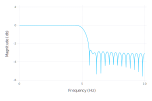
\includegraphics[width=\linewidth]{/home/travis/build/mpastell/Weave.jl/doc/build/examples/tmpXzW0HU/FIR_design_4_1.pdf}

And again with default options


\begin{lstlisting}
(*@\HLJLn{h{\_}phase}@*) (*@\HLJLoB{=}@*) (*@\HLJLnf{unwrap}@*)(*@\HLJLp{(}@*)(*@\HLJLoB{-}@*)(*@\HLJLn{atan}@*)(*@\HLJLoB{.}@*)(*@\HLJLp{(}@*)(*@\HLJLn{imag}@*)(*@\HLJLoB{.}@*)(*@\HLJLp{(}@*)(*@\HLJLn{h}@*)(*@\HLJLp{),}@*)(*@\HLJLn{real}@*)(*@\HLJLoB{.}@*)(*@\HLJLp{(}@*)(*@\HLJLn{h}@*)(*@\HLJLp{)))}@*)
(*@\HLJLnf{plot}@*)(*@\HLJLp{(}@*)(*@\HLJLn{ws}@*)(*@\HLJLp{,}@*) (*@\HLJLn{h{\_}phase}@*)(*@\HLJLp{,}@*)
    (*@\HLJLn{xlabel}@*) (*@\HLJLoB{=}@*) (*@\HLJLs{"Frequency (Hz)"}@*)(*@\HLJLp{,}@*) (*@\HLJLn{ylabel}@*) (*@\HLJLoB{=}@*) (*@\HLJLs{"Phase (radians)"}@*)(*@\HLJLp{)}@*)
\end{lstlisting}

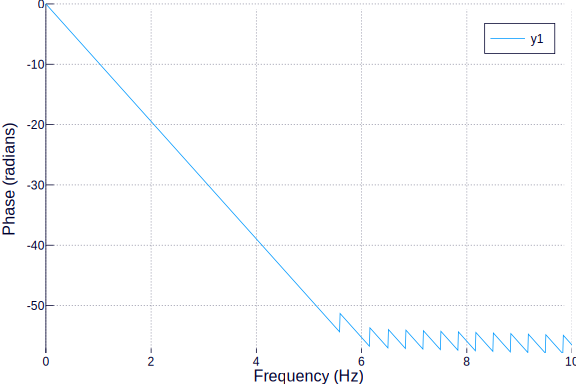
\includegraphics[width=\linewidth]{/home/travis/build/mpastell/Weave.jl/doc/build/examples/tmpXzW0HU/FIR_design_5_1.pdf}


\end{document}
